\hypertarget{introduction}{%
\section{Introduction}\label{introduction5}}

Epithelial structures in biology exhibit a diverse range of shapes and sizes, including curved or folded forms. Understanding these structures can be complicated, particularly in the context of developmental biology. Interestingly, the etymology of the terms "development" and "complicated" provides insight into the importance of folding and unfolding processes. "Development" comes from "desvelopemens," meaning "unfolding," which describes the morphogenesis of an organism. In contrast, "complicated" comes from "com-plicare," meaning "folded together," which is fitting for describing the emergence of complex, folded structures in epithelial tissues.

In our experimental system, 3D epithelial structures can be generated by inflating domes, transforming a planar monolayer into a curved structure. In this chapter, we will discuss how these structures can be made even more "complicated". By studying the mechanics of epithelial tissue, we have discovered that the dome can be deflated into folds by rapidly depressurizing it. We will explore the process of epithelial buckling and discuss how this knowledge has enabled us to transform domes into folded structures.

\hypertarget{rapid-deflation-produces-a-buckling-instability}{%
	\section{Rapid deflation produces a buckling
		instability}\label{rapid-deflation-produces-a-buckling-instability}}

\begin{figure}
	\centering
	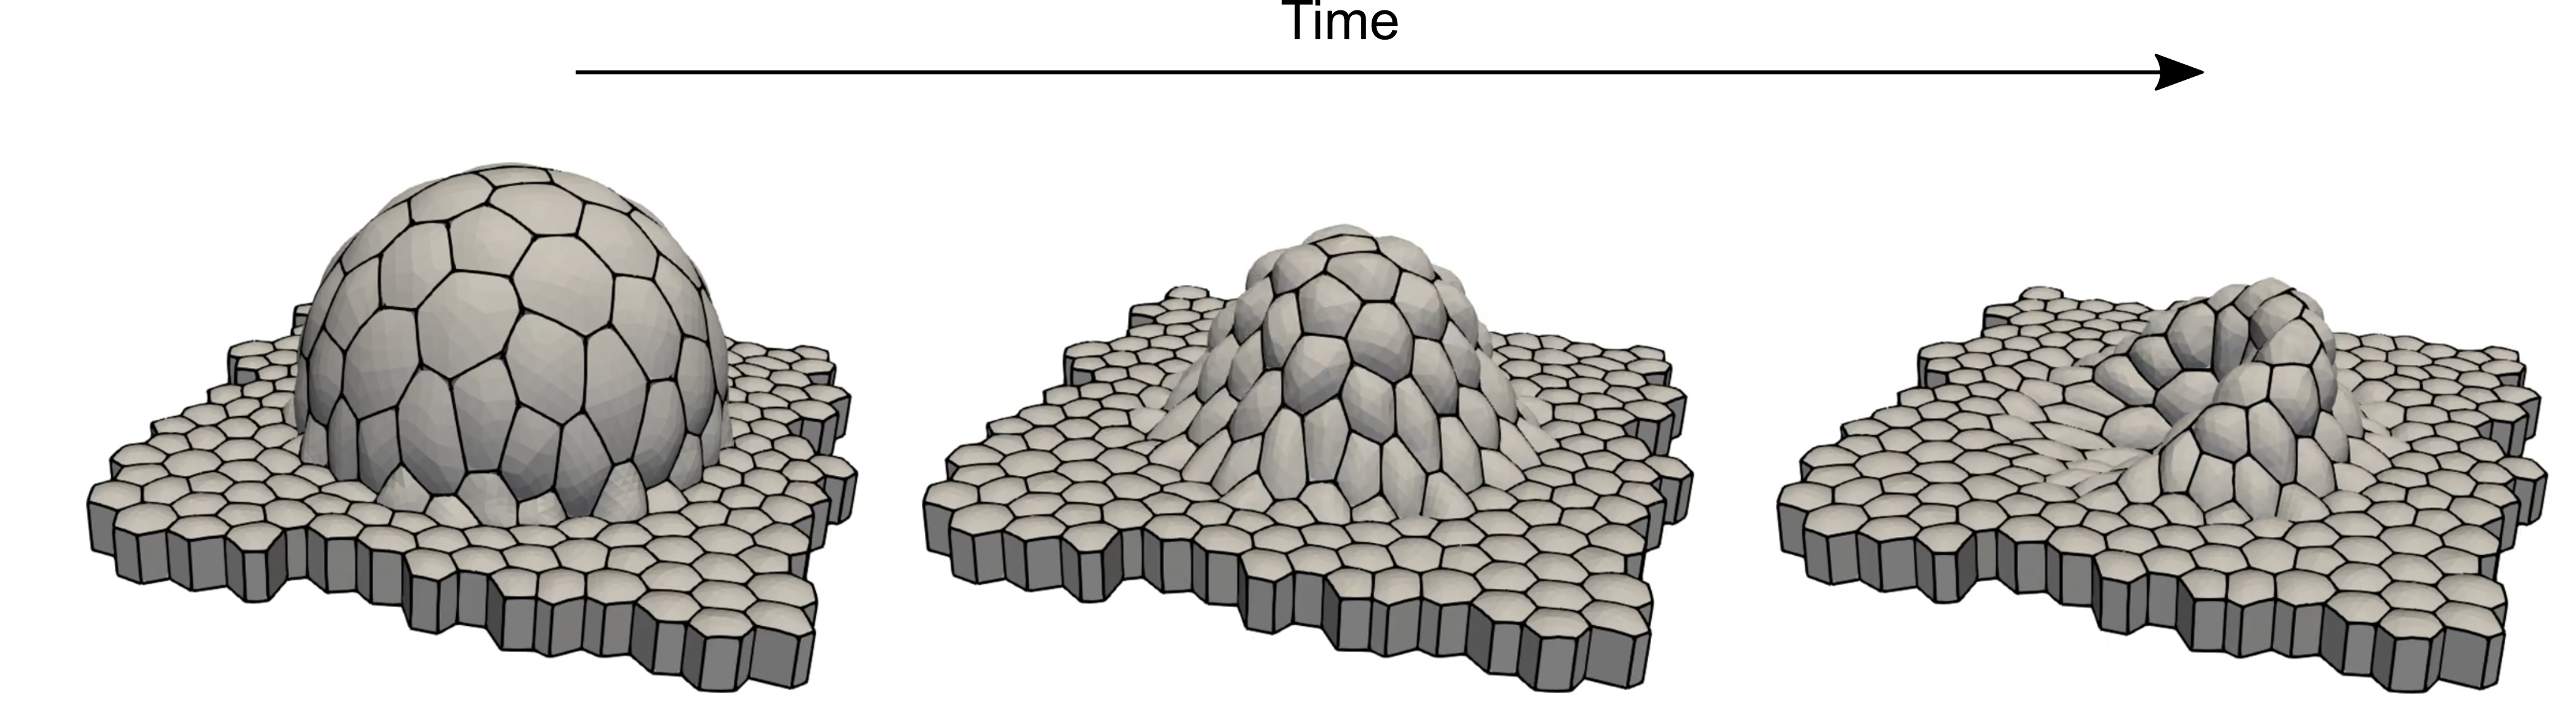
\includegraphics[width=\textwidth]{chap8_digitaldome.png}
	\caption{\label{fig_8_1} \textbf{Digital dome undergoing buckling}:Here, a digital dome at a steady state is rapidly deflated to a negative pressure of $-50Pa$. As the cells don't have enough time to reduce their area, they collapse into a fold.
	}
\end{figure}

In our experiments involving constant pressure, we observed that the dome reached a steady state through cytoskeletal remodeling. Specifically, the original footprint area increased to areal strains exceeding $100\%$, more than double the original area. Moreover, when subjected to cyclic stretching, we observed that rapid inflation-deflation cycles accumulated strains in the tissue. Given our precise control over pressure, we decided to expose the tissue to extreme rates of pressure, allowing no time for relaxation and could lead to buckling instability.

First by using the computational model, we were able to examine the mechanical effects of the digital dome on both tissue and cell scales. Our analysis revealed that active viscoelastic dissipation through cortical remodeling allowed the dome to achieve high strains. When we subjected the dome to cyclic stretching at rapid rates, we noticed a discrepancy between the actual and resting areas. This observation suggested that fast deflation could induce negative viscoelastic stress, leading to buckling. 

Our findings showed that digital domes gradually returned to a flat monolayer when deflated at a rate slower than the remodeling timescale. However, deflating the domes more quickly than the remodeling timescales resulted in buckling (see fig \ref{fig_8_1}). Simulations revealed that the negative pressure was necessary for inducing buckling, which affected only rapidly deflating domes. This was due to negative stresses, as the pressure became negative while the curvature remained positive. In contrast, slowly deflating domes reached zero strain as the pressure approached zero.

To systematically test our hypothesis regarding the factors affecting buckling events, we designed experiments with pressure profiles consisting of three stages (see fig \ref{fig_8_2}). Firstly, we initiated a linear increase in pressure from 0 to 200 Pa over a period of 10 seconds. Secondly, we applied constant pressure for varying "hold times," which were chosen based on the timescales associated with actomyosin cytoskeletal remodeling. Finally, we decreased the pressure to -50Pa at varying "deflation rates."

\begin{figure}
	\begin{minipage}[c]{0.6\textwidth}
		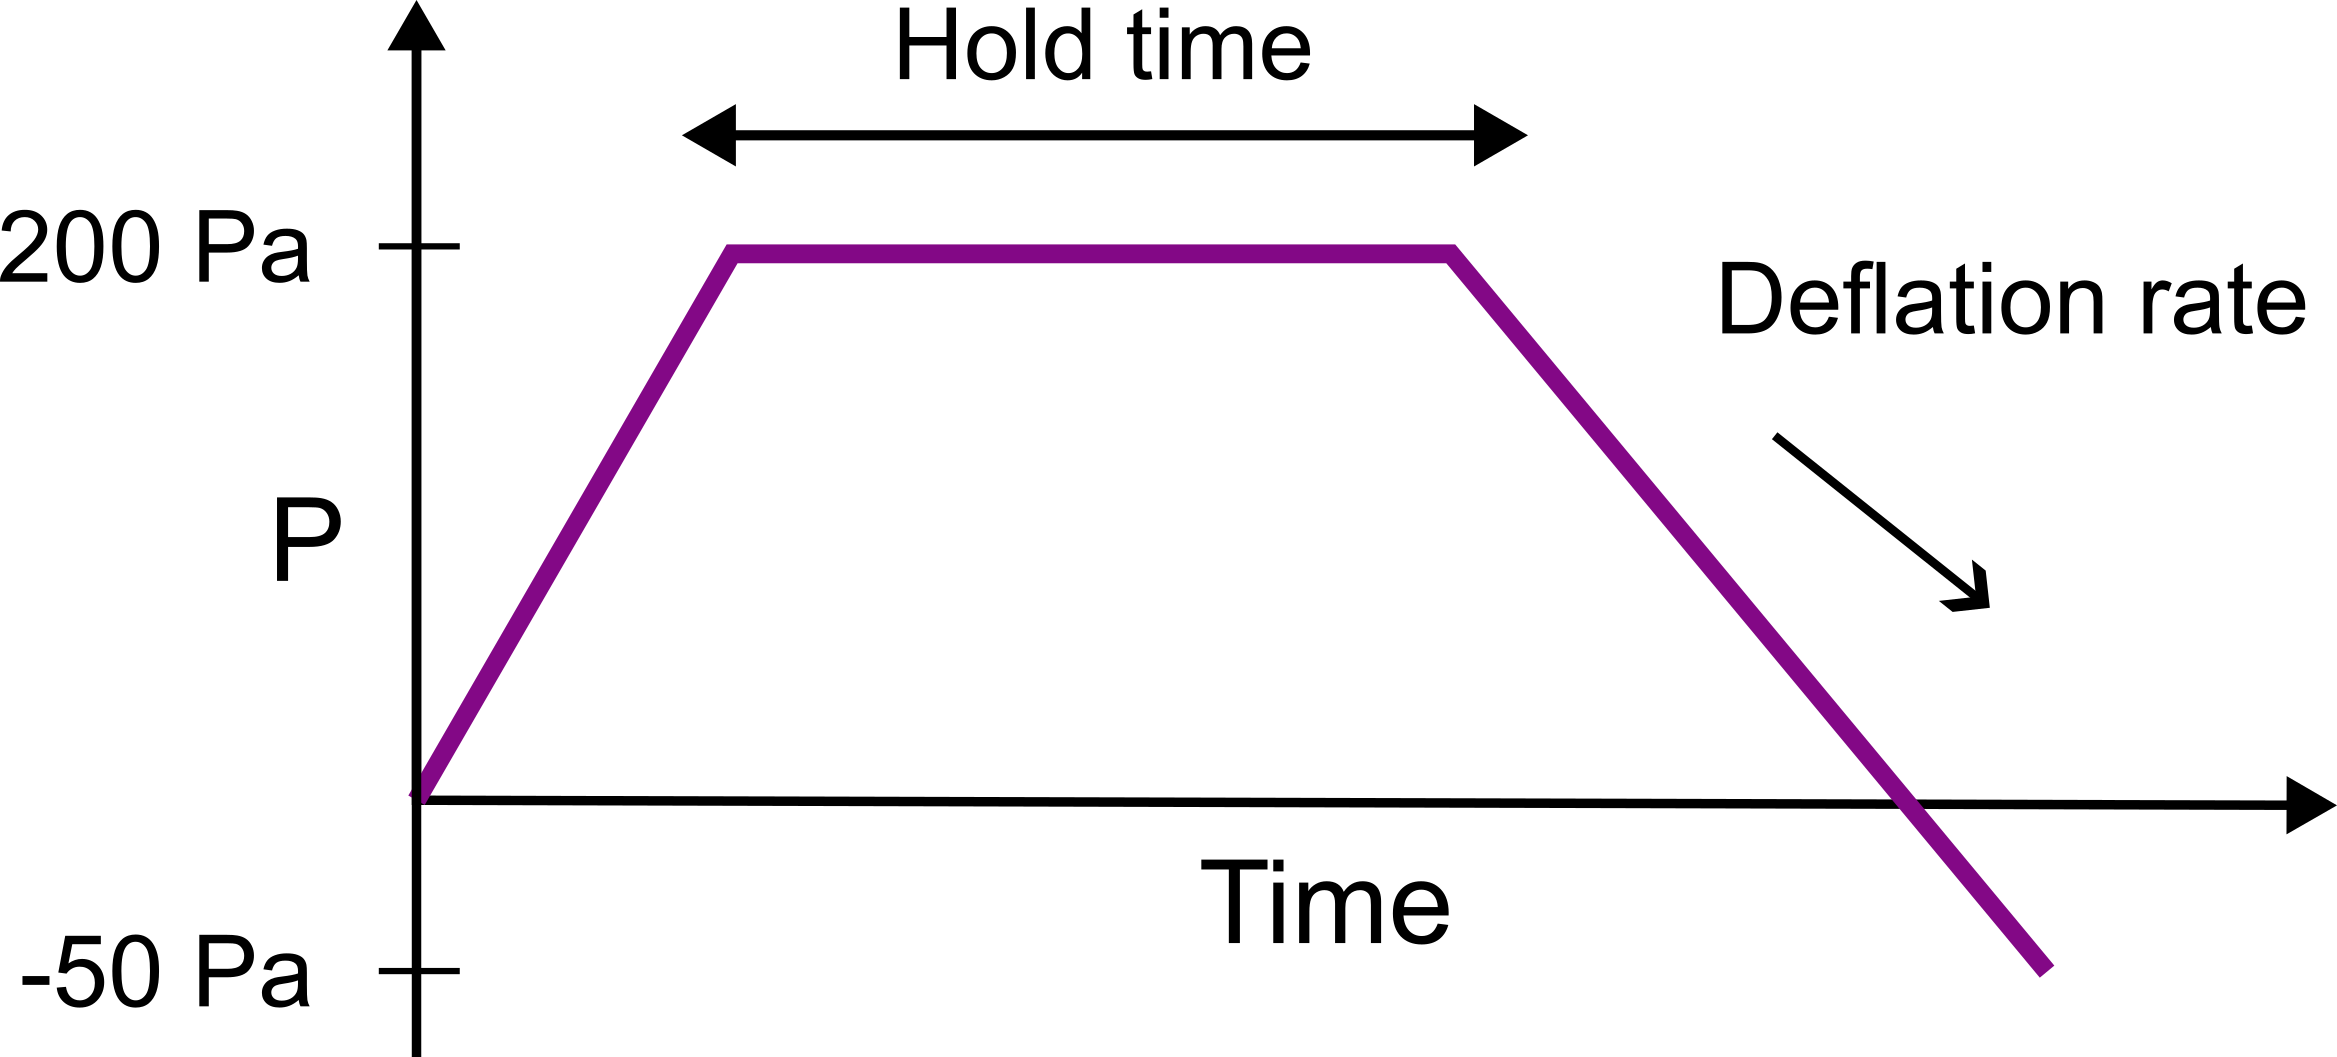
\includegraphics[width=\textwidth]{chap8_bucklingprotocol.png}
	\end{minipage}\hfill
	\begin{minipage}[c]{0.35\textwidth}
		\caption{\\ \textbf{Buckling protocol}:\\ The pressure is increased to 200Pa for inflating the dome, and then the dome is given different amounts of time (hold time) to remodel before being deflated to -50Pa at different rates (deflation rate) to observe whether the dome buckles or not.	} \label{fig_8_2}
	\end{minipage}
\end{figure}

It is important to note that we relied on qualitative characterization of buckling events, assuming that smooth and continuous curvature of the monolayer indicates the absence of buckling. However, in cases where it was difficult to make an unbiased judgment, we enlisted the help of Thomas Wilson and Tom Golde to categorize the data. We performed the experiments for all conditions and quantified the data by tracking the fraction of domes that underwent buckling.

Our results showed that buckling occurred for all hold times, ranging from 6s to 600s, at the fastest deflation rate of 200 Pa/s. This confirmed our hypothesis that rapid deflation would induce compressive stresses and cause buckling (see fig \ref{fig_8_3} A-B). On the other hand, slow deflation at a rate of 0.2 Pa/s rarely led to buckling, regardless of the hold time (see fig \ref{fig_8_3} C-D). This suggests that the tissue can effectively remodel its cytoskeleton and adapt to drastic changes in area to avoid buckling.

As seen in previous experiments, longer "hold times" allowed for more cytoskeletal remodeling, resulting in higher strains and a higher likelihood of buckling, even for slower deflation rates. Results plotted in a phase diagram illustrates the trend: as hold time increases, buckling becomes more likely at faster deflation rates and less likely at slower deflation rates with a shorter hold time (see fig \ref{fig_8_3} E).

Interestingly, the data showed that domes with a 6s hold time had smaller strains compared to those with a 600s hold time, which is consistent with results from domes subjected to constant pressure (see fig \ref{fig_8_3} F). Strain increase requires time for the dome to remodel and balance active tension with the externally applied pressure. However, even at 6s hold time, we still observed buckling. Expectation for this condition was to allow us for inflation and deflation of the dome before it could remodel. We selected a 6s hold time based on imaging speeds, but it remained too slow for the remodeling timescales.

It is important to note that we observed a wide variety of buckling patterns when examining midsections of the tissue through a line scan method. Some domes exhibited minor kinks in the folds, while others showed drastic buckling modes similar to those of plates.

\begin{figure}[h]
	\centering
	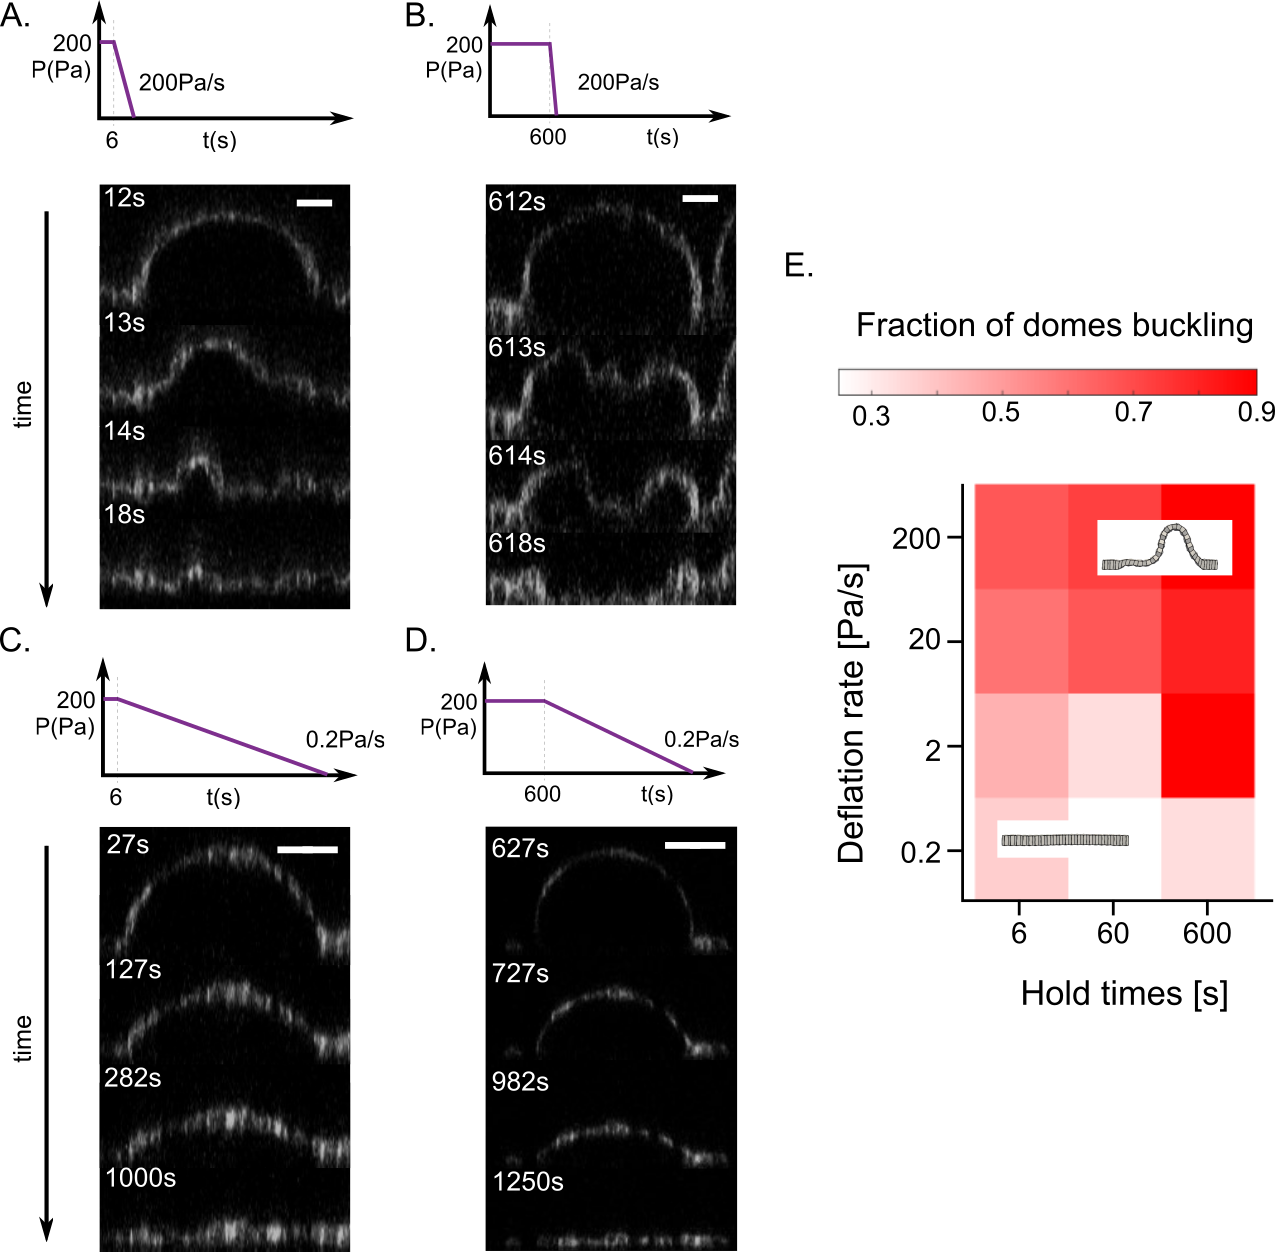
\includegraphics[width=\textwidth]{chap8_buckling.png}
	\caption{\label{fig_8_3} \textbf{Buckling conditions}: (A-D) Representative montages of dome deflation for experiments and model at different deflation rates of 200 and 0.2 Pa/s after holding pressure constant of 200 Pa for 6 and 600 s. Scale bars are 20 µm for XZ. (E) Diagram representing fraction of domes buckling for different deflation rates and hold time. Showing the optimum conditions for the buckling. (F) The maximum strain achieved is lower for 6s hold time compared to 600s conditions.
	}
\end{figure}


\hypertarget{multiscale-buckling}{%
	\section{Multiscale buckling}\label{multiscale-buckling}}

\begin{figure}
	\centering
	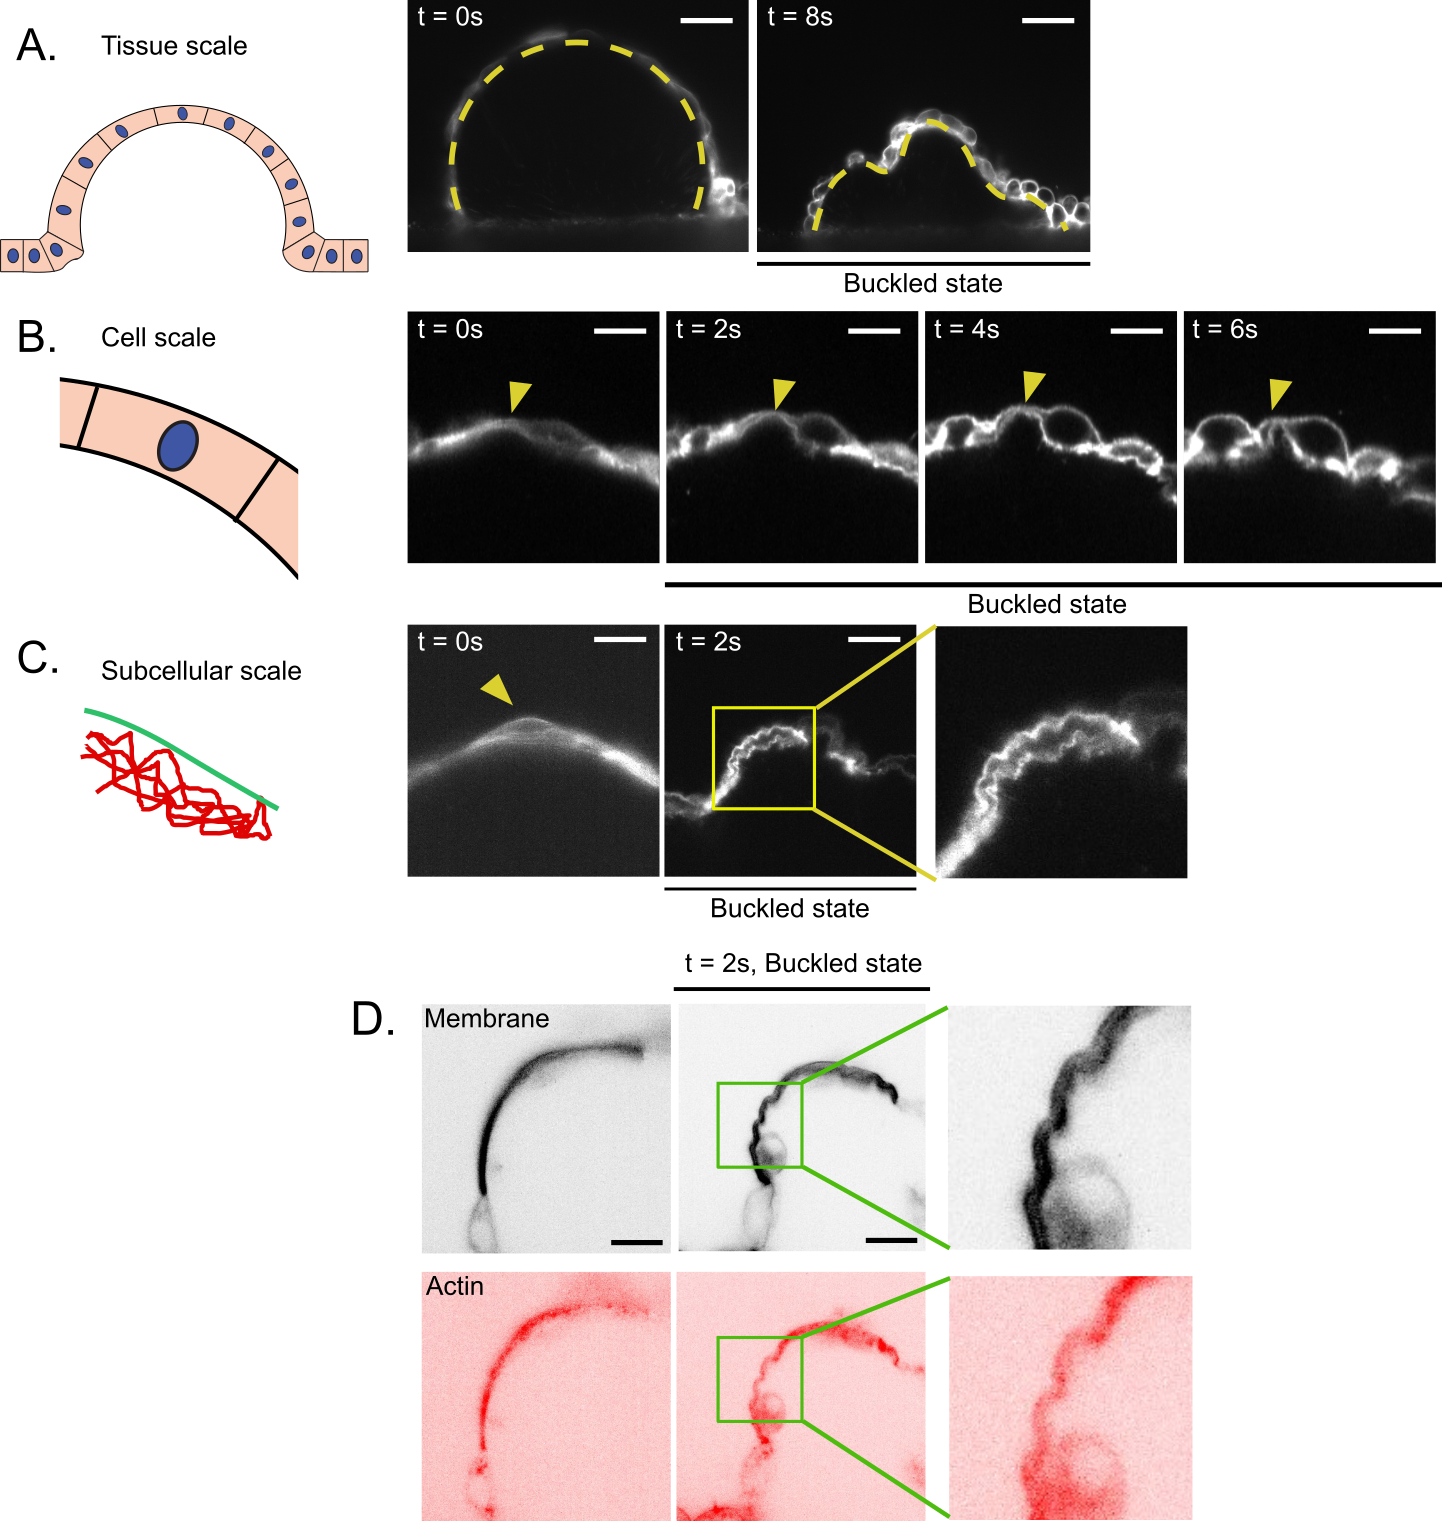
\includegraphics[width=\textwidth]{chap8_bucklingmultiscale.png}
	\caption{\label{fig_8_4} \textbf{Multiscale buckling}: (A-C) Representative images of the domes undergoing buckling at different scales. Buckled and unbuckled states of the dome with zoom in section buckled component. Dotted yellow line represents uniform curvature in unbuckled state and non-uniform curvature in buckled state. Scale bar is $20 \mu m$. (B) Evolution of a single cell in the dome during buckling. Highlighted by yellow arrow. (C) Some parts of cells undergo buckling producing short wavelength folds. (D) These  folds are also present in the cortex too. Scale bar is $5 \mu m$ for (B-D).
	}
\end{figure}

The observation of tissue buckling was evident in the confocal line scan images. In order to gain a clearer understanding of the shape of the cells, we adapted a variation of MOLI for use with light sheet microscopy. The higher resolution 3D images of the dome revealed a variety of thicknesses, with thicker regions caused by the bulging of the nucleus and very thin regions at the cell periphery (see fig \ref{fig_8_6} B).

To further investigate the phenomenon of buckling, we repeated the experiments described in the previous section, this time with rapid deflation and a long hold time. We discovered additional features beyond tissue-scale buckling, including kinks and crimps at cellular and subcellular scales. Upon closer inspection, we classified three levels of buckling:

At the tissue scale, buckling was visible with cells collectively transitioning from a uniform curvature to a distorted shape (see fig \ref{fig_8_6} A). At this level, we observed cell deformation at a larger scale, including at the junctions between cells.

At shorter scales, we observed individual cells undergoing buckling (see fig \ref{fig_8_6} B). The buckling of the cell resulted in the cell doubling up around itself, with the apical side at the top. The length scale at which cell buckling occurred was much shorter than that observed at the tissue level. It appears as though the cell buckles as a single unit.

In some cases, buckling occurred at even shorter length scales, which we refer to as subcellular buckling, as the folds in the membrane were distinct from the cell level buckling. These folds occurred in the thinnest parts of the stretched cells, where the membrane buckled at much shorter wavelengths (see fig \ref{fig_8_6} C). Interestingly, these folds occurred on both the apical and basal sides of the cells.

\begin{figure}[h!]
	\centering
	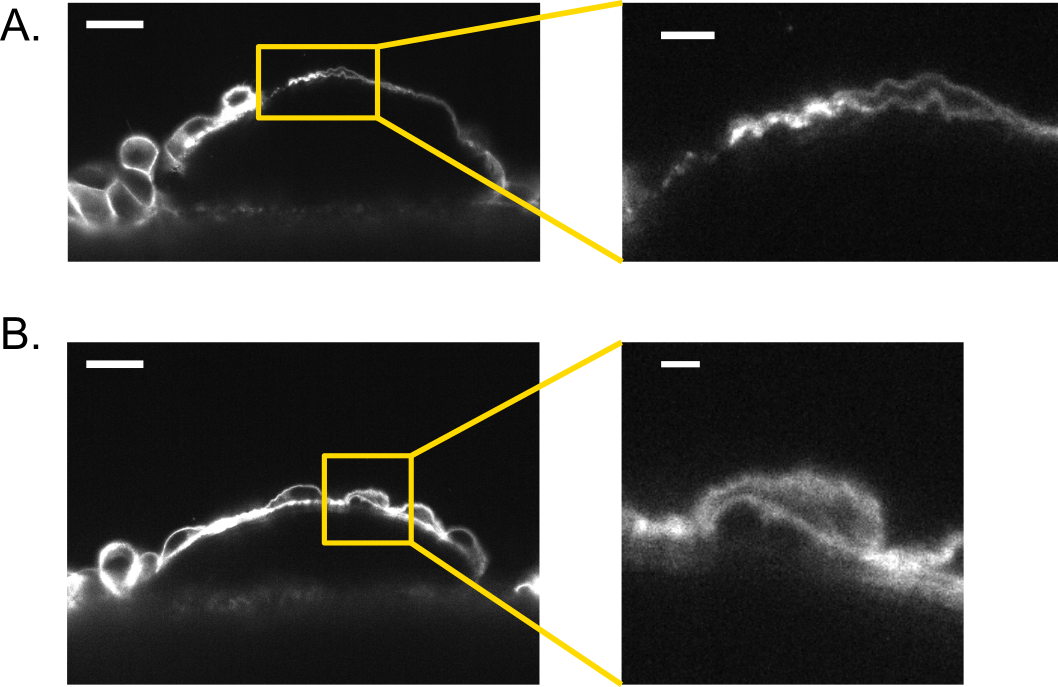
\includegraphics[width=0.8\textwidth]{chap8actinbuckling.png}
	\caption{\label{fig_8_6} \textbf{Cell level buckling}: In many instances where the tissue does not buckle, we observe individual cells buckling. Here is an example of cell buckling (A) and subcellular buckling (B).}
\end{figure}

In epithelial cells, the membrane is typically attached to the cortex through membrane-cortex attachment proteins such as ezrin, radixin, and moesin. It is reasonable to assume that the subcellular buckling observed in our experiments is due to actin cortex buckling. To confirm this, we imaged the actin cortex while the dome was undergoing buckling using SPY actin staining (see fig \ref{fig_8_6} D). Our results showed that the actin cortex followed the exact shape of the membrane during buckling.

We also observed interesting results where some domes did not appear to be buckling at the tissue scale, but were still exhibiting buckling at the cell or subcellular level (see fig \ref{fig_8_7}). These categories are not strictly separated, as we observed multiple instances of tissue, cell, and subcellular level buckling (see fig \ref{fig_8_6} A).


\hypertarget{generating-epithelial-folds}{%
	\section{Generating epithelial
		folds}\label{generating-epithelial-folds}}

After optimizing the buckling conditions, we embarked on exploring epithelial folds. We have been imaging only the cross-section of the dome to capture the fast dynamics. We see the buckling in form of the squiggly lines. However, these buckling events are three-dimensional (see fig \ref{fig_8_3} B). During tissue buckling, a large area squeezed into original footprint area resulted in the formation of folds and wrinkles in the monolayer. Monitoring the base of the dome deflating, we observed that the tissue made contact with the substrate in certain regions first and others later. This led to the formation of folds in the regions where it made contact last (see fig \ref{fig_8_5} A-C).

To investigate if there was any pattern to these folds, we looked at spherical domes of various sizes. Broadly, we observed three types of folding patterns emerging (see fig \ref{fig_8_8}):

\begin{figure}[h!]
	\begin{minipage}[c]{0.5\textwidth}
		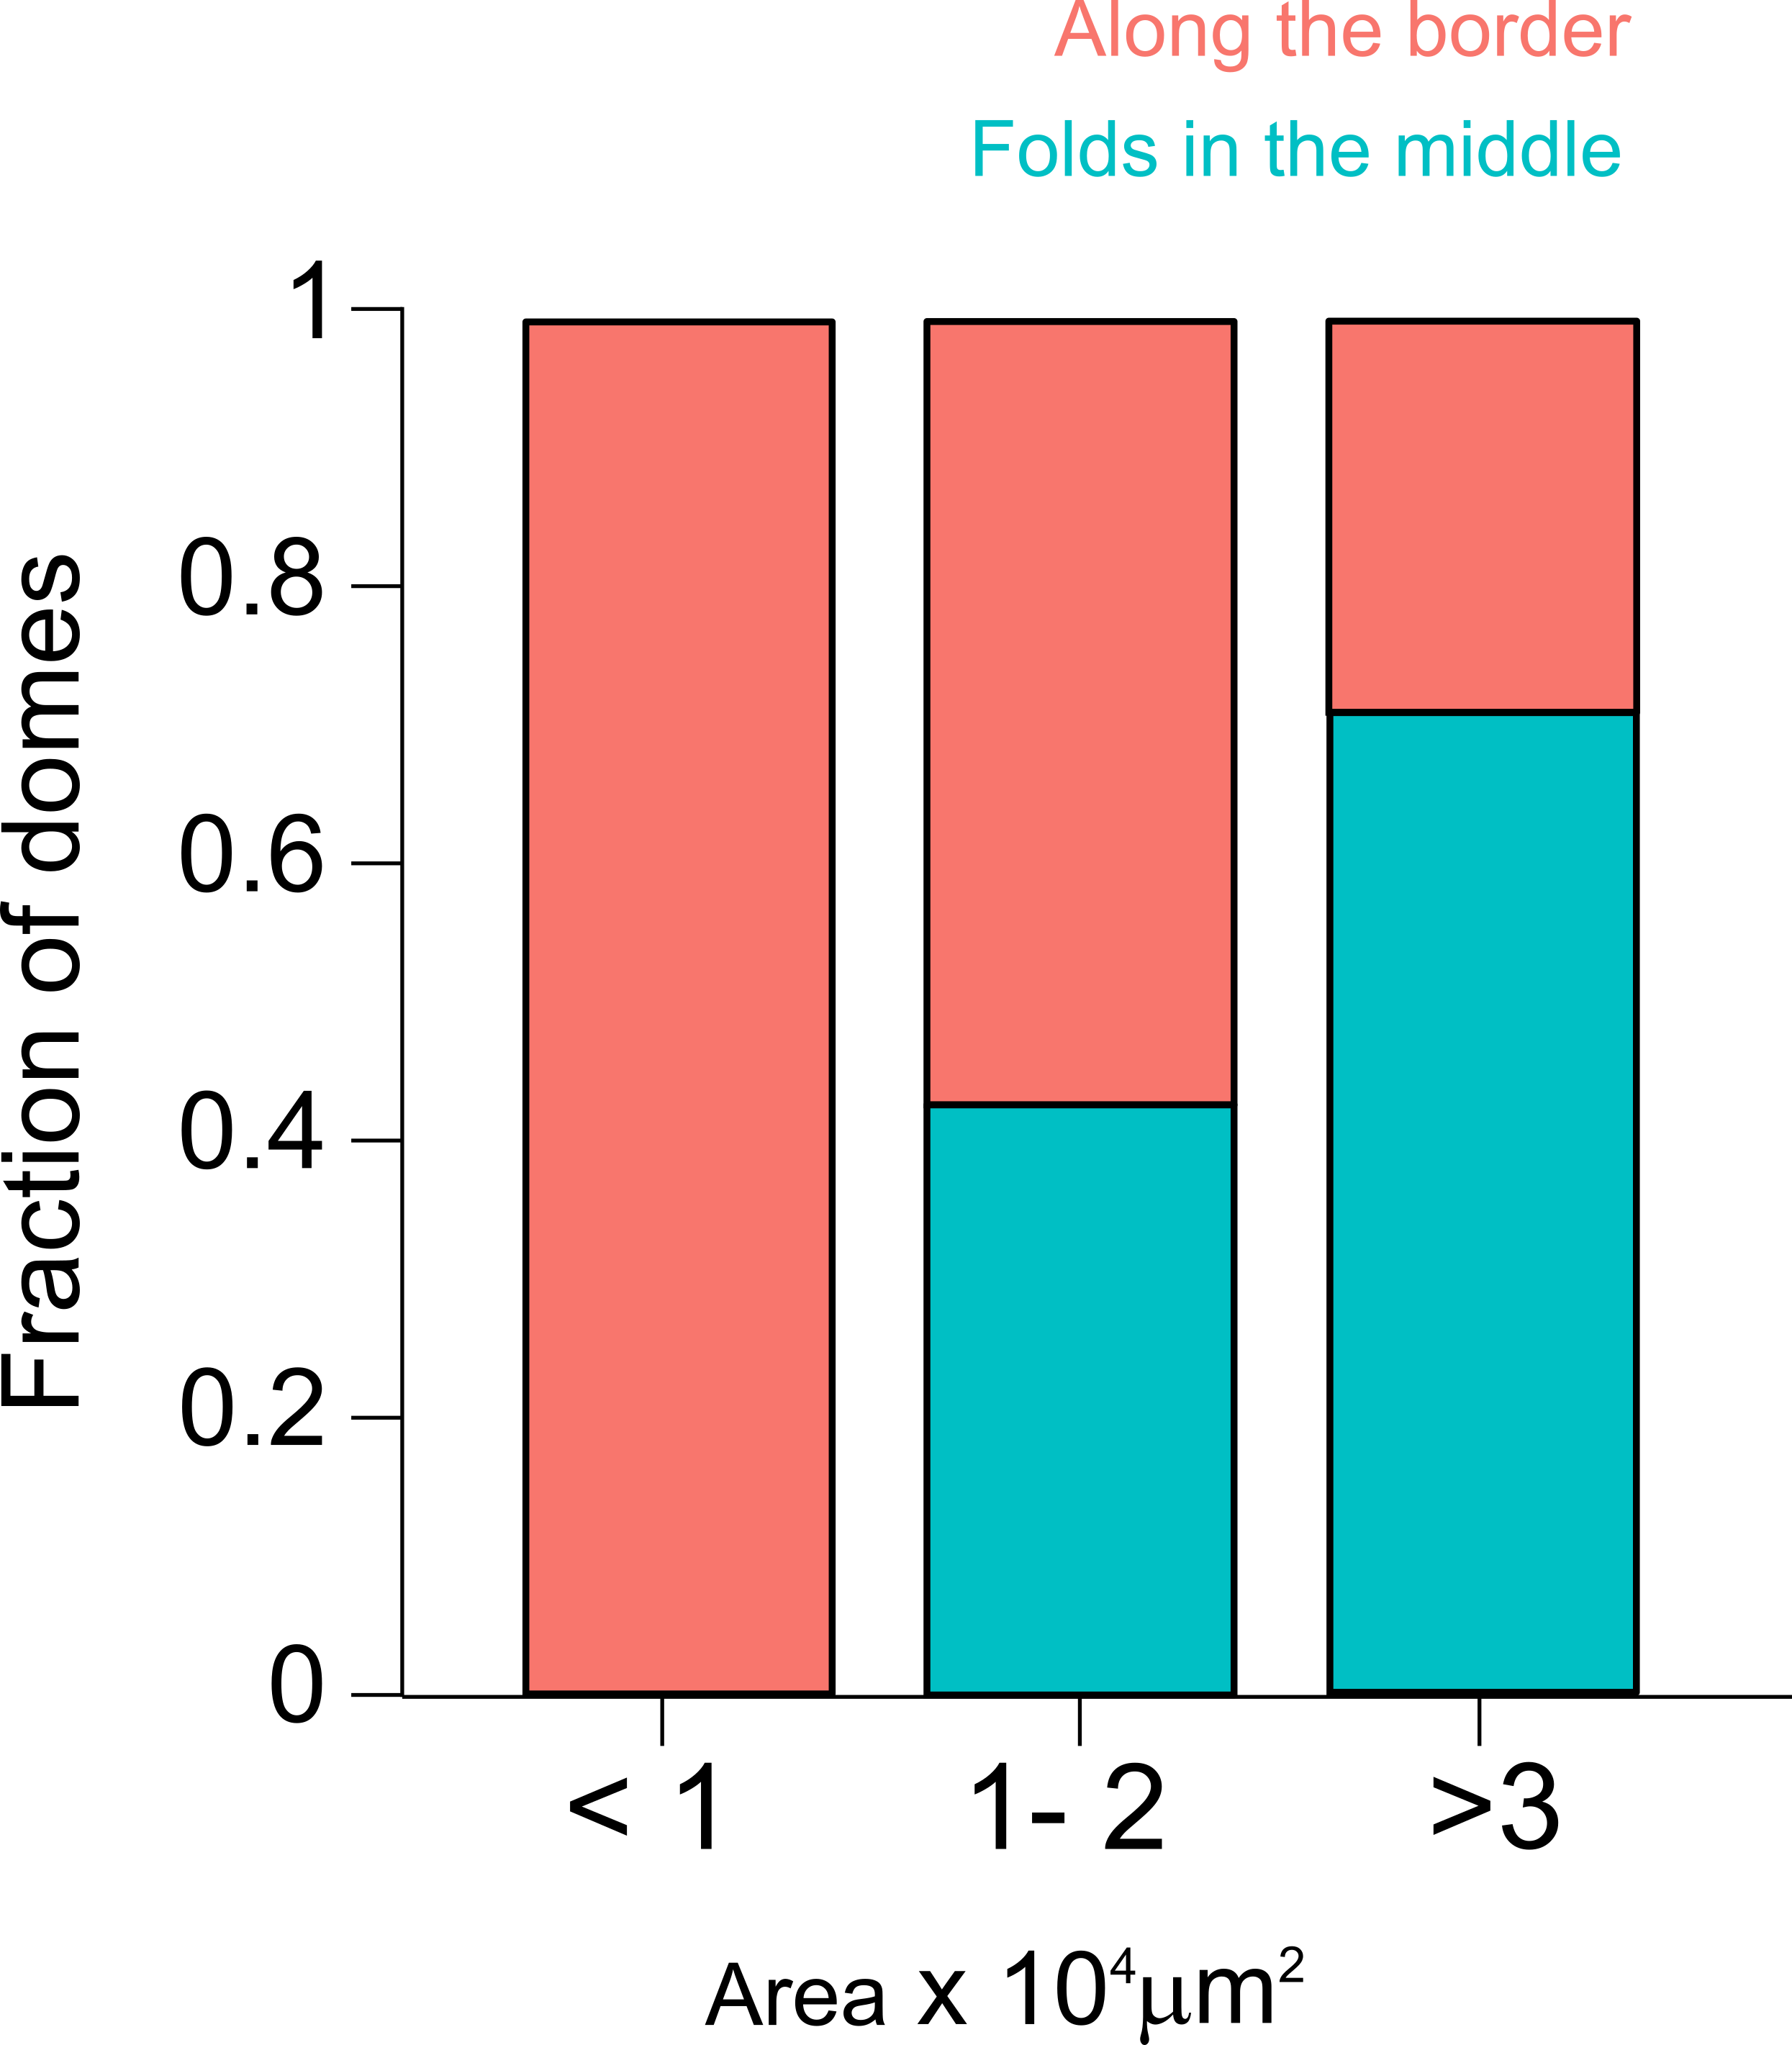
\includegraphics[width=0.8\textwidth]{chap8patternfraction.png}
	\end{minipage}\hfill
	\begin{minipage}[c]{0.45\textwidth}
		\caption{\\ \textbf{Buckling patterns}:\\ 
		Buckling patterns observed in differently sized digital domes. The domes were grouped into three size categories and two categories based on location of folds (along the border and in the middle). We found that larger domes are more likely to buckle into a network of folds compared to smaller ones.
		} \label{fig_8_8}
	\end{minipage}
\end{figure}

For domes with a footprint diameter smaller than $\sim 110 \mu m$, we repeatedly observed that most of the buckling resulted in an accumulation around the periphery (see fig \ref{fig_8_5} A). The confocal timelapse from the base gave the impression of a donut-like structure, but three-dimensional imaging of the folds revealed a crescent-shaped fold like a croissant, taller on one side than the other. For larger domes with a footprint  diameter greater than $\sim 300 \mu m$, we observed more instances of domes forming a network of folds in the middle, with multiple folds connecting each other by forming junctions (see fig \ref{fig_8_5} C). Finally, for domes of intermediate size, we observed a mixture of accumulation and folds, although the proportion of folds along the periphery decreased (see fig \ref{fig_8_8}).

Interestingly, we observed the same folding patterns in our digital domes when performing the same deflation experiments (see fig \ref{fig_8_5} D). Larger digital domes produced more radial folds, and small digital domes formed an accumulation on the side. Intermediate-sized digital domes showed a mixture of both patterns.

\begin{figure}
	\centering
	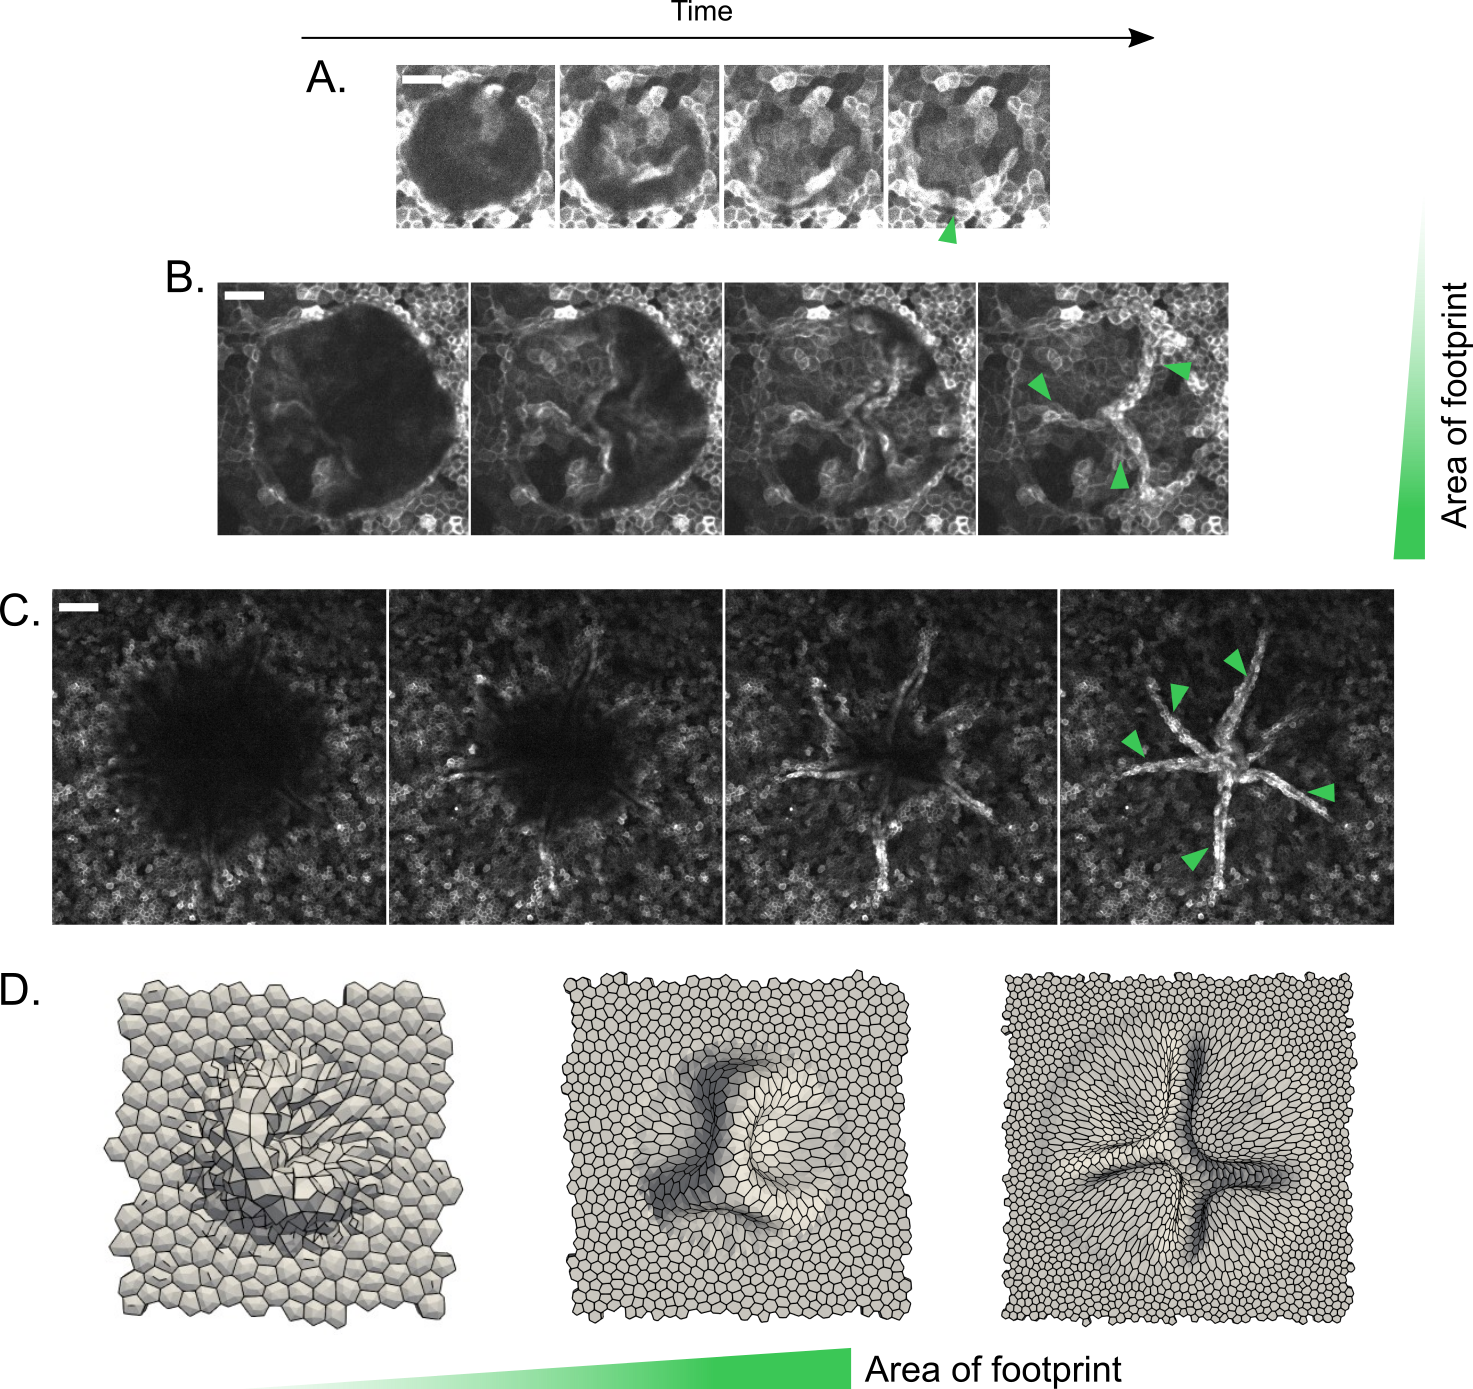
\includegraphics[width=\textwidth]{chap8_bucklingfolds.png}
	\caption{\label{fig_8_5} \textbf{Buckling patterns in spherical domes of varied size}: Representative examples of digital domes undergoing buckling with time-lapse of their basal cross-section (A-C). In the first frame, the onset of buckling is visible where the dome makes contact in the middle. Subsequent frames show more of the fold coming into view, and when the dome completely deflates, a fold is formed (indicated by the green arrow). Panel (D) shows the final outcome of buckling for digital domes of different sizes. Scale bar is $20 \mu m$	}
\end{figure}

\hypertarget{forming-predictable-folds}{%
	\section{Forming predictable folds}\label{forming-predictable-folds}}

We were curious about how the geometry of the domes could affect the pattern formation of folds. Although we observed that different sizes of spherical domes produced different beautiful buckling patterns, the axis-symmetric shape made it difficult to predict the patterns. To address this, we decided to generate ellipsoidal domes of different sizes using MOLI. Interestingly, we found that the ellipsoidal domes would buckle into a fold along their major axis, with smaller ellipsoidal domes producing a similar peripheral accumulation as spherical domes and larger ellipsoidal domes producing a fold in the center along the major axis (see fig \ref{fig_8_7} B). This suggested that only larger domes, regardless of their shape, could produce folds.

To further explore the possibility of creating more complex folds, we decided to buckle a dome with a triangular shape, anticipating that the vertices of the triangle could push the buckling along the medians of the triangle (see fig \ref{fig_8_7} C). As expected, the domes did buckle into forming a Y-shaped network of the fold (see fig \ref{fig_8_7} D). We also repeated the triangular and ellipsoidal shapes with digital domes and found similar patterns (see fig \ref{fig_8_7} A-B).

We also investigated the stability of these folded structures. We found that not all folds were alike, some would dissipate into the monolayer while others would last longer by forming attachments with each other, and they were stable for hours and could be imaged for more than 12 hours (see fig \ref{fig_8_7} E-F). Interestingly, if immediately inflated these folds would unfurl themselves into a dome again.

These results suggest that the MOLI system could provide a novel way of producing folds, with potential applications in tissue engineering, by simply controlling a few mechanical parameters such as geometry and pressure.

\begin{figure}
	\centering
	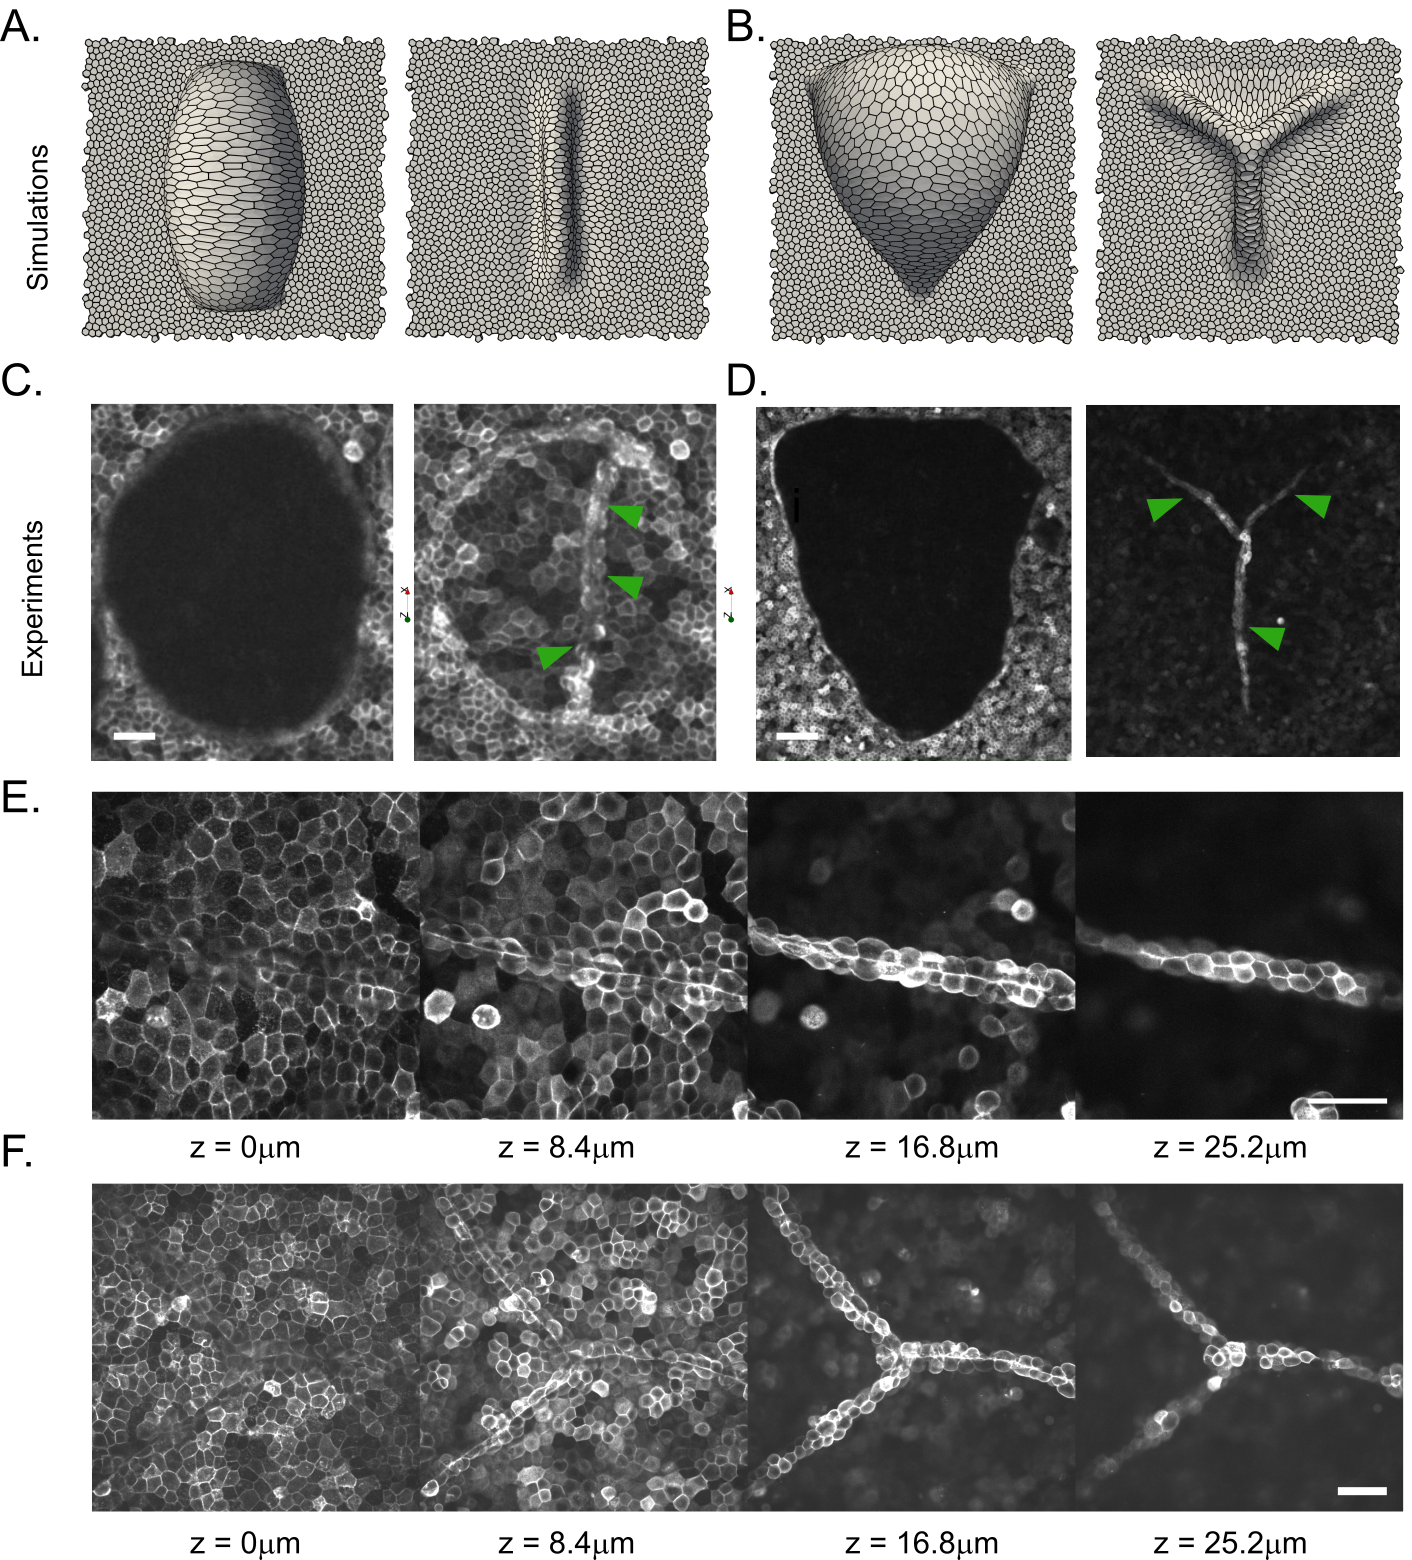
\includegraphics[width=\textwidth]{chap8_pfolds.png}
	\caption{\label{fig_8_7} \textbf{Controling the patterns of fold}: A-B Simulations show digital models of ellipsoidal and triangular domes buckled into line and Y-shaped junctions. C-D Experimental results confirm the simulation findings. E-F Confocal z-stack images show the folds in the case of a line and Y-shaped junction. Scale bar is $50\mu m$.	}
\end{figure}


\newpage
\hypertarget{summary-and-discussion-1}{%
	\section{Summary and Discussion}\label{summary-and-discussion-1}}

We utilized our device to generate dome from a flat monolayer then transform it into folds, alongside investigating the buckling response in relation to actin remodeling timescales. We discovered that buckling occurs at various scales, starting from the tissue level down to the actin cortex of individual cells, and is triggered when deflation occurs more rapidly than actin can remodel. We then explored the patterns of folding that emerge from different sized and shaped domes, and proposed a new method of creating controlled folds from planar monolayer. With the aid of computational models, we demonstrated the engineering potential of the dome system to produce structured folds by manipulating the geometry and pressure.

As mentioned earlier, mechanical instabilities are ubiquitous in biological systems, and the phenomenon of buckling has been observed in MDCK epithelial monolayers through various methods, such as growth in confinement or direct application of compression \cite{wyatt2020,trushko2020}. Wyatt et al. demonstrated that compressive stress greater than 35\% strain can cause epithelial monolayers to buckle out of plane, and showed that active contractility can recover the out-of-plane deformation within tens of seconds.

Our study, on the other hand, is the first to offer visual insights into the minute details of the buckling process and its implications for tissue architecture at multiple scales.

From a mechanistic perspective, our result are a consequence of the hierarchical structure of the epithelial tissue, which comprises various components that sustain deformations and forces at different levels. Notably, the actin cytoskeleton plays a critical role in defining the shape of cells and tissues at multiple scales  \cite{clarke2021}. Additionally, a cell monolayer can be considered as an assembly of cells with their own surface tension and material properties, indicating a material with different length scales would buckle at different length scales. Therefore, if there is a local weakness in a cell or subcellular feature, it is expected to locally buckle. For instance, we only observed subcellular-level buckling in very thin cells while overall tissue doesn't buckle.

Furthermore, the short-wavelength folds resulting from subcellular buckling are intriguing to consider. It is worth noting that actin buckling is not a new phenomenon in the field, and there are minimal models of actin filaments with myosin motors on a lipid membrane demonstrating that myosin-induced contraction leads to actin filament buckling \cite{murrell2012, costa2002,  wang2019}. In membrane-actin droplets, researchers have reported multiple modes in the form of buckling and wrinkling, depending on the thickness \cite{kusters2019}. Interestingly, they found that thin shells undergo buckling and thin shells produce wrinkles in the membrane but not in actin, which could indicate different modes of buckling within a cell.

In the context of tissue-scale buckling, our results can be understood in terms of modes of buckling in thin shells. Our computational model suggests that the cortex behaves like a hyperelastic material, as evidenced by the rate at which we are deflating these tissues. Similar results would be obtained if we repeated the experiment with elastic shells. The literature on thin shell buckling reveals similar aspects, such as the folds and patterns that emerge when different sized shells buckle.

The slenderness, defined as the ratio of dome radius to thickness, intuitively guides the different modes of buckling. Thin shells with high slenderness would lead to a higher mode of buckling compared to thicker shells. However, our experiments go beyond understanding the system and show that we can program folds by minimally controlling two parameters: geometry and pressure. For non-spherical domes, anisotropic stresses are observed along the axes of the elliptical footprint for ellipsoidal domes. These stresses can orient the folding in a particular direction to generate a programmed fold, such as Y junctions on the sides of a rectangular footprint.

In summary, this thesis presents a novel experimental system that allows us to inflate epithelial domes and deflate them into tubes. We demonstrate that the timescales of actomyosin cytoskeleton remodeling play a key role in this transformation. By controlling the geometry of the epithelia and the rate of deflation, we show that we can engineer epithelial folds of desired geometry.